% Options for packages loaded elsewhere
\PassOptionsToPackage{unicode}{hyperref}
\PassOptionsToPackage{hyphens}{url}
\PassOptionsToPackage{dvipsnames,svgnames,x11names}{xcolor}
\documentclass[
  spanish,
  10pt,
  a4paper,
]{article}
\usepackage{xcolor}
\usepackage[top=22mm,bottom=22mm,left=22mm,right=22mm]{geometry}
\usepackage{amsmath,amssymb}
\setcounter{secnumdepth}{-\maxdimen} % remove section numbering
\usepackage{iftex}
\ifPDFTeX
  \usepackage[T1]{fontenc}
  \usepackage[utf8]{inputenc}
  \usepackage{textcomp} % provide euro and other symbols
\else % if luatex or xetex
  \usepackage{unicode-math} % this also loads fontspec
  \defaultfontfeatures{Scale=MatchLowercase}
  \defaultfontfeatures[\rmfamily]{Ligatures=TeX,Scale=1}
\fi
\usepackage{lmodern}
\ifPDFTeX\else
  % xetex/luatex font selection
\fi
% Use upquote if available, for straight quotes in verbatim environments
\IfFileExists{upquote.sty}{\usepackage{upquote}}{}
\IfFileExists{microtype.sty}{% use microtype if available
  \usepackage[]{microtype}
  \UseMicrotypeSet[protrusion]{basicmath} % disable protrusion for tt fonts
}{}
\usepackage{setspace}
\makeatletter
\@ifundefined{KOMAClassName}{% if non-KOMA class
  \IfFileExists{parskip.sty}{%
    \usepackage{parskip}
  }{% else
    \setlength{\parindent}{0pt}
    \setlength{\parskip}{6pt plus 2pt minus 1pt}}
}{% if KOMA class
  \KOMAoptions{parskip=half}}
\makeatother
\usepackage{longtable,booktabs,array}
\newcounter{none} % for unnumbered tables
\usepackage{calc} % for calculating minipage widths
% Correct order of tables after \paragraph or \subparagraph
\usepackage{etoolbox}
\makeatletter
\patchcmd\longtable{\par}{\if@noskipsec\mbox{}\fi\par}{}{}
\makeatother
% Allow footnotes in longtable head/foot
\IfFileExists{footnotehyper.sty}{\usepackage{footnotehyper}}{\usepackage{footnote}}
\makesavenoteenv{longtable}
\usepackage{graphicx}
\makeatletter
\newsavebox\pandoc@box
\newcommand*\pandocbounded[1]{% scales image to fit in text height/width
  \sbox\pandoc@box{#1}%
  \Gscale@div\@tempa{\textheight}{\dimexpr\ht\pandoc@box+\dp\pandoc@box\relax}%
  \Gscale@div\@tempb{\linewidth}{\wd\pandoc@box}%
  \ifdim\@tempb\p@<\@tempa\p@\let\@tempa\@tempb\fi% select the smaller of both
  \ifdim\@tempa\p@<\p@\scalebox{\@tempa}{\usebox\pandoc@box}%
  \else\usebox{\pandoc@box}%
  \fi%
}
% Set default figure placement to htbp
\def\fps@figure{htbp}
\makeatother
\ifLuaTeX
\usepackage[bidi=basic,shorthands=off]{babel}
\else
\usepackage[bidi=default,shorthands=off]{babel}
\fi
\ifLuaTeX
  \usepackage{selnolig} % disable illegal ligatures
\fi
\setlength{\emergencystretch}{3em} % prevent overfull lines
\providecommand{\tightlist}{%
  \setlength{\itemsep}{0pt}\setlength{\parskip}{0pt}}

\usepackage{amsmath,amssymb,mathtools}
\usepackage{microtype}
\usepackage{fancyhdr}
\usepackage{needspace}
\usepackage{etoolbox}
\usepackage{float}
\usepackage{caption}
\captionsetup{font=small,labelformat=empty,skip=7pt}
\floatplacement{figure}{H}
\definecolor{DocBlue}{HTML}{173F57}
\definecolor{DocGray}{HTML}{52616C}
\pagestyle{fancy}
\fancyhf{}
\fancyhead[L]{\small\sffamily\color{DocGray} pySNSPD | Desarrollo del modelo}
\fancyhead[R]{\small\sffamily\color{DocGray} Revisión 0.2}
\fancyfoot[L]{\small\sffamily\color{DocGray} 8 de septiembre de 2026}
\fancyfoot[R]{\small\sffamily\thepage}
\setlength{\headheight}{15pt}
\setlength{\emergencystretch}{2em}
\setlength{\parskip}{5pt plus 1pt}
\setlength{\parindent}{0pt}
\widowpenalty=10000
\clubpenalty=10000
\displaywidowpenalty=10000
\predisplaypenalty=10000
\renewcommand{\arraystretch}{1.16}
\AtBeginEnvironment{longtable}{\small}
\pretocmd{\section}{\Needspace{6\baselineskip}}{}{}
\pretocmd{\subsection}{\Needspace{5\baselineskip}}{}{}
\AtBeginDocument{\hypersetup{colorlinks=true,linkcolor=DocBlue,urlcolor=DocBlue}}
\allowdisplaybreaks[1]
\usepackage{bookmark}
\IfFileExists{xurl.sty}{\usepackage{xurl}}{} % add URL line breaks if available
\urlstyle{same}
\hypersetup{
  pdftitle={D. Síntesis{,} plan y verificaciones},
  pdflang={es},
  colorlinks=true,
  linkcolor={Maroon},
  filecolor={Maroon},
  citecolor={Blue},
  urlcolor={Blue},
  pdfcreator={LaTeX via pandoc}}

\title{D. Síntesis, plan y verificaciones}
\usepackage{etoolbox}
\makeatletter
\providecommand{\subtitle}[1]{% add subtitle to \maketitle
  \apptocmd{\@title}{\par {\large #1 \par}}{}{}
}
\makeatother
\subtitle{Actualización del modelo pySNSPD · Documento 4 de 4}
\author{}
\date{8 de septiembre de 2026 · Revisión 0.2}

\begin{document}
\maketitle

{
\setcounter{tocdepth}{2}
\tableofcontents
}
\setstretch{1.07}
\newpage

\section{D.0. Qué cambia en esta
iteración}\label{d.0.-quuxe9-cambia-en-esta-iteraciuxf3n}

El objetivo es ampliar las capacidades de modelamiento de SNSPD:
conectar mejor el espectro, la redistribución de energía, la respuesta
del condensado y la señal eléctrica. La descripción quasiclásica
proporciona herramientas para esa mejora sin exigir una reconstrucción
exacta de todos los procesos de la materia condensada.

La revisión 0.2 conserva la propuesta de A--C y corrige una afirmación
de alcance de la versión anterior. \textbf{El uso de corriente Usadel en
el cierre modificado tiene una justificación explícita de continuidad.}
Vodolazov la desarrolla mediante un término adicional en el lado derecho
de la ecuación de orden; la memoria muestra su cancelación algebraica en
el anexo C. La comparación entre cierres uniformes cuantifica
diferencias entre aproximaciones. Por sí sola no demuestra que la
corriente anterior sea inválida {[}M, V{]}.

El funcional común se estudia como una ampliación útil para derivar
fuerzas y almacenamiento energético con convenciones compartidas. Su
beneficio debe comprobarse en los observables del detector. La versión
0.2 desarrolla la derivación desde {[}F{]}, añade figuras reproducibles
y explica la relación entre energía y temperatura. \textbf{En C se
conserva la formulación dinámica propuesta para continuar su revisión.}
Los ejemplos añadidos no introducen una nueva movilidad de producción ni
una predicción nueva de latencia.

{\def\LTcaptype{none} % do not increment counter
\begin{longtable}[]{@{}
  >{\raggedright\arraybackslash}p{(\linewidth - 4\tabcolsep) * \real{0.3333}}
  >{\raggedright\arraybackslash}p{(\linewidth - 4\tabcolsep) * \real{0.3333}}
  >{\raggedright\arraybackslash}p{(\linewidth - 4\tabcolsep) * \real{0.3333}}@{}}
\toprule\noalign{}
\begin{minipage}[b]{\linewidth}\raggedright
Documento
\end{minipage} & \begin{minipage}[b]{\linewidth}\raggedright
Cambio principal de la revisión 0.2
\end{minipage} & \begin{minipage}[b]{\linewidth}\raggedright
Pregunta que permite contestar
\end{minipage} \\
\midrule\noalign{}
\endhead
\bottomrule\noalign{}
\endlastfoot
A & Derivación desde {[}F{]}, teorema de la envolvente explícito,
corrección del juicio sobre la corriente & ¿Qué energía se varía y qué
se mantiene fijo? \\
B & Figuras de reacciones, inversión térmica y poblaciones de igual
energía & ¿Qué conserva un balance y qué información pierde una
temperatura? \\
C & Explicación de las coordenadas energéticas y ejemplos de relajación
y circuito & ¿Por qué aparece una temperatura y cómo se forma la tensión
del puerto? \\
D & Síntesis, pruebas de esta versión y plan actualizado & ¿Qué está
verificado y qué falta antes de cambiar producción? \\
\end{longtable}
}

\section{D.1. Tres distinciones que ordenan el
modelo}\label{d.1.-tres-distinciones-que-ordenan-el-modelo}

\subsection{D.1.1. Continuidad de corriente y energía
común}\label{d.1.1.-continuidad-de-corriente-y-energuxeda-comuxfan}

La continuidad responde a una pregunta local: si entra carga en una
región, ¿sale la misma carga bajo la aproximación cuasineutra? El
término correctivo de Vodolazov y su implementación en la memoria
atienden esta pregunta. La construcción de A responde además a otra: ¿la
fuerza de amplitud y la corriente pueden calcularse como pendientes de
una energía electrónica común?

Una analogía útil es una red de tuberías. Cumplir el balance de caudales
en cada unión es una condición física; conocer también cuánto trabajo
almacena o libera el sistema requiere una relación constitutiva
adicional. La analogía solo separa las dos preguntas: no identifica
corriente superconductora con flujo hidráulico ni decide qué cierre
dinámico es mejor.

Para el funcional reducido de A, las identidades son

\[
\begin{gathered}
X_{|\Delta|}^{\rm FD}
=\left.\frac{\partial f_e^{\rm FD}}{\partial |\Delta|}\right|_{T,\mathbf q}
=2N_0G,\\
\boldsymbol\Pi^{\rm FD}
=\left.\frac{\partial f_e^{\rm FD}}{\partial\mathbf q}\right|_{T,|\Delta|}
=\frac{\hbar}{2e}\mathbf j_s.
\end{gathered}\tag{D.1}
\]

Su identidad de derivadas mixtas, en una rama suave y con una dirección
fija de corriente, es

\[
\frac{\partial X_{|\Delta|}^{\rm FD}}{\partial q}
=\frac{\hbar}{2e}\frac{\partial j_s}{\partial|\Delta|}.
\tag{D.2}
\]

D.2 comprueba la construcción termodinámica uniforme; la conservación de
carga sigue siendo una ecuación que debe cumplir el sistema espacial.
Ninguna de estas pruebas, aislada, valida la movilidad, los vórtices o
la latencia a baja temperatura.

\subsection{D.1.2. Energía electrónica y energía de
excitaciones}\label{d.1.2.-energuxeda-electruxf3nica-y-energuxeda-de-excitaciones}

La energía libre de A describe el sector electrónico efectivo: incluye
el cambio asociado al emparejamiento y a las excitaciones, con
referencia explícita al metal normal. No es únicamente una integral de
energía de cuasipartículas ni la energía total de iones, electrones,
campos y circuito.

En la extensión adiabática a ocupaciones no térmicas se usa

\[
\begin{gathered}
u_e=U_{\rm vac}(|\Delta|,q)+u_{\rm qp},\\
u_{\rm qp}=4N_0\int_0^\infty E\rho(E;|\Delta|,q)f(E)\,dE.
\end{gathered}\tag{D.3}
\]

Aquí \(N_0\) es la DOS normal por espín; el factor cuatro sigue las
convenciones de excitaciones positivas de A. El término de vacío
superconductivo ya contiene su dependencia del superflujo. Añadir una
segunda energía local del mismo superflujo contaría dos veces ese
almacenamiento. Los fonones y la inductancia exterior tienen balances
separados, unidos por potencias que se intercambian con signos opuestos.

\subsection{D.1.3. Coordenada energética y cierre
térmico}\label{d.1.3.-coordenada-energuxe9tica-y-cierre-tuxe9rmico}

Es posible avanzar numéricamente \(u_{\rm qp}\) y consultar una
temperatura equivalente cuando un coeficiente o una figura la requiera.
A espectro fijo se define el mapa

\[
\begin{gathered}
u_{\rm qp}=\mathcal U(T_E;|\Delta|,q),\\
\mathcal U(T;|\Delta|,q)=4N_0\int_0^\infty
\frac{E\rho(E;|\Delta|,q)}{e^{E/(k_BT)}+1}\,dE,\\
C_{\rm qp}=\left.\partial_T\mathcal U\right|_{|\Delta|,q}>0.
\end{gathered}\tag{D.4}
\]

La inversa es única dentro del intervalo energético representado. Esto
establece una correspondencia entre \textbf{dos coordenadas escalares},
con \(|\Delta|\) y \(q\) fijados. No establece una correspondencia entre
la temperatura y todas las distribuciones posibles. Una mochila puede
pesar lo mismo con contenidos diferentes; conocer el peso no determina
qué objeto hay dentro. De forma análoga, la energía total no determina
las poblaciones que intervienen en las fuerzas o colisiones.

Si cambia el espectro, la regla de la cadena da

\[
\dot u_{\rm qp}=C_{\rm qp}\dot T_E
+\left.\partial_{|\Delta|}\mathcal U\right|_{T_E,q}\partial_t|\Delta|
+\left.\partial_{\mathbf q}\mathcal U\right|_{T_E,|\Delta|}\cdot\dot{\mathbf q}.
\tag{D.5}
\]

Por ello ni \(u_{\rm qp}\) ni \(T_E\) pueden convertirse con una tabla
unidimensional fija cuando varían \(|\Delta|\) o \(q\). Al avanzar
energía electrónica total también debe contabilizarse \(U_{\rm vac}\).
Las formas de C en temperatura conservan utilidad para mostrar esta
transformación; no obligan a seleccionar temperatura como incógnita
primaria del futuro algoritmo.

La hipótesis térmica aparece al sustituir la distribución por
\(f_{\rm FD}(T_E)\) en las fuerzas y tasas. Esa sustitución requiere
pruebas sobre corriente, fuerza, intercambio y transporte. La igualdad
de energía, impuesta por D.4, no sirve como prueba independiente del
cierre.

\section{D.2. Cómo se conectan las capas de
A--C}\label{d.2.-cuxf3mo-se-conectan-las-capas-de-ac}

El estado espectral temprano y el estado térmico reducido son dos
representaciones con distinto contenido. El paso de una a otra se acepta
cuando las magnitudes relevantes dejan de distinguirlas dentro de
tolerancias declaradas.

{\def\LTcaptype{none} % do not increment counter
\begin{longtable}[]{@{}
  >{\raggedright\arraybackslash}p{(\linewidth - 4\tabcolsep) * \real{0.3333}}
  >{\raggedright\arraybackslash}p{(\linewidth - 4\tabcolsep) * \real{0.3333}}
  >{\raggedright\arraybackslash}p{(\linewidth - 4\tabcolsep) * \real{0.3333}}@{}}
\toprule\noalign{}
\begin{minipage}[b]{\linewidth}\raggedright
Capa
\end{minipage} & \begin{minipage}[b]{\linewidth}\raggedright
Variables y operaciones
\end{minipage} & \begin{minipage}[b]{\linewidth}\raggedright
Información que entrega a la siguiente capa
\end{minipage} \\
\midrule\noalign{}
\endhead
\bottomrule\noalign{}
\endlastfoot
Material & \(D,\sigma_n,N_0,T_c,F,\alpha^2F\), convenciones de energía y
modos & Escalas y pesos de transporte e interacción \\
Espectro instantáneo, A & Resolver Usadel con \(|\Delta|\) y
\(\mathbf q\) dados & DOS y funciones anómalas; borde espectral y
respuesta de corriente \\
Poblaciones, B & Evolucionar ocupaciones, fuentes, transporte y
colisiones & Energía, fuerza no térmica, corriente e intercambio
electrón--fonón \\
Condensado, C & Usar fuerzas y movilidad declarada; resolver continuidad
& Amplitud, fase, campo eléctrico y trabajo interno \\
Exterior y circuito, C & Acoplar calor, corriente e inductancia con el
dominio local & Realimentación y tensión en el puerto elegido \\
\end{longtable}
}

\subsection{D.2.1. Balance que debe conservar cualquier
reducción}\label{d.2.1.-balance-que-debe-conservar-cualquier-reducciuxf3n}

Cada reacción electrón--fonón transfiere la misma energía que retira del
otro subsistema. Para una celda con espectro fijo y únicamente esas
colisiones,

\[
\dot u_e\big|_{e\text{-ph}}=-P_{e\text{-ph}},\qquad
\dot u_{\rm ph}\big|_{e\text{-ph}}=+P_{e\text{-ph}}.
\tag{D.6}
\]

La cancelación sobrevive a distribuciones no térmicas. Un discretizado
por bandas debe retirar y añadir la misma energía por evento. Ajustar
por separado dos tablas de potencia que casi coincidan es una
verificación más débil que conservar esa estructura desde las
reacciones.

En la extensión espacial propuesta, la energía total local satisface el
balance de C.18:

\[
\begin{aligned}
\partial_t\big(u_e+K_0|\nabla|\Delta||^2+u_{\rm ph}\big)
={}&-\nabla\cdot\mathbf Q_e+\nabla\cdot\mathbf J_{\rm tr}\\
&+\mathbf j_{\rm tot}\cdot\mathbf E-P_{\rm esc}+S_\gamma^{(E)}.
\end{aligned}\tag{D.7}
\]

La corriente de transporte energético \(\mathbf J_{\rm tr}\) se define
en C a partir del trabajo del condensado. El campo eléctrico
\(\mathbf E\) es un vector y no debe confundirse con la energía
espectral escalar \(E\). Integrar D.7 sobre el dominio convierte las
divergencias en flujos de borde: así se prueba si el dominio pequeño
entrega al exterior el calor y el trabajo correctos.

La disipación del condensado de C es

\[
Q_\Delta=\Gamma_{|\Delta|}(\partial_t|\Delta|)^2
+\Gamma_\theta\left(\dot\theta+\frac{2e}{\hbar}\phi\right)^2\geq0.
\tag{D.8}
\]

Representa transferencia a los grados de libertad disipativos. No es una
creación adicional de energía que se pueda sumar dos veces al balance
total. La positividad de la movilidad es una condición del cierre; su
magnitud y su validez durante un estado no térmico siguen pendientes de
contraste.

\subsection{D.2.2. Señal que se desea
modelar}\label{d.2.2.-seuxf1al-que-se-desea-modelar}

Para la topología de fuente de corriente y carga física de C,

\[
\begin{gathered}
L_{\rm ext}^{\rm diff}\dot I+V_{\rm patch}=R_L(I_b-I),\\
V_{\rm port}=R_L(I_b-I).
\end{gathered}\tag{D.9}
\]

La tensión del dominio local y la del puerto pueden diferir durante la
redistribución de corriente. Una respuesta calculada con resistencia
prescrita sirve para entender esa diferencia y verificar el circuito; no
calcula cuándo se formó dicha resistencia tras absorber un fotón.

El objetivo de desarrollo continúa siendo una absorción declarada hasta
el pico de tensión previo al amplificador, con la realimentación física
de la carga. Se deben distinguir el tiempo de cambio local del
condensado, un phase slip, la formación de una franja resistiva, el
cruce de un umbral de puerto y el pico. La revisión 0.2 no agrega una
predicción de eficiencia, conteos oscuros o distribución estadística de
jitter.

\section{D.3. Resultados reproducidos en la versión
0.2}\label{d.3.-resultados-reproducidos-en-la-versiuxf3n-0.2}

\subsection{D.3.1. Equilibrio uniforme en
Geminga}\label{d.3.1.-equilibrio-uniforme-en-geminga}

Se reejecutó un cálculo independiente del transiente de producción,
usando \(T=0.9\) K, \(T_c=8.65\) K, \(D=1.581\times10^{-4}\) m\(^2\)/s,
\(\sigma_n=4.2\times10^5\) S/m, ancho de 120 nm y espesor de 7 nm. El
barrido resuelve problemas algebraicos uniformes y usa colas asintóticas
de Matsubara hasta orden \(\epsilon_n^{-4}\).

{\def\LTcaptype{none} % do not increment counter
\begin{longtable}[]{@{}
  >{\raggedright\arraybackslash}p{(\linewidth - 4\tabcolsep) * \real{0.3333}}
  >{\raggedleft\arraybackslash}p{(\linewidth - 4\tabcolsep) * \real{0.3333}}
  >{\raggedleft\arraybackslash}p{(\linewidth - 4\tabcolsep) * \real{0.3333}}@{}}
\toprule\noalign{}
\begin{minipage}[b]{\linewidth}\raggedright
Cierre uniforme
\end{minipage} & \begin{minipage}[b]{\linewidth}\raggedleft
Máximo de corriente
\end{minipage} & \begin{minipage}[b]{\linewidth}\raggedleft
Diferencia respecto de Usadel
\end{minipage} \\
\midrule\noalign{}
\endhead
\bottomrule\noalign{}
\endlastfoot
Usadel: amplitud autoconsistente y corriente & 38.850324 µA &
Referencia \\
Amplitud Allmaras y corriente Usadel & 35.182843 µA & −9.44\% \\
Amplitud Allmaras y corriente aproximada de Vodolazov & 40.143624 µA &
+3.33\% \\
\end{longtable}
}

\begin{figure}
\centering
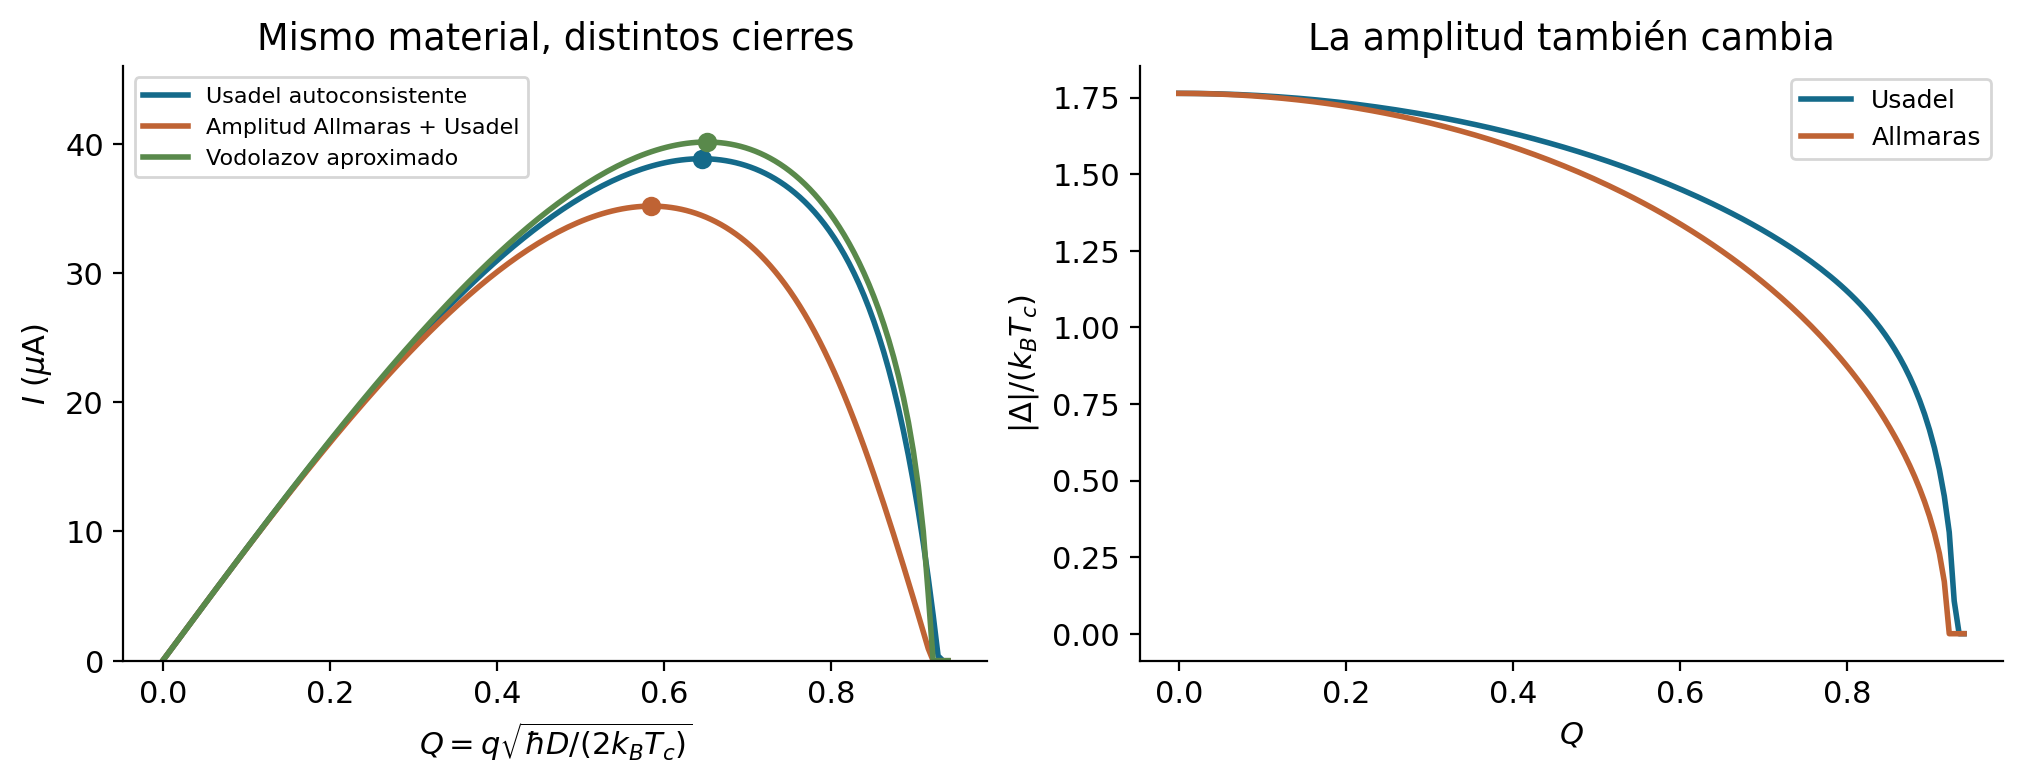
\includegraphics[width=1\linewidth,height=\textheight,keepaspectratio,alt={Figura D.1. Resultado cuantitativo uniforme, reproducido en esta revisión. A la izquierda se comparan corrientes; a la derecha, las amplitudes que alimentan esas corrientes. Un máximo de estas ramas no es la corriente de switching de un nanohilo finito.}]{../figuras/A_02_corriente_uniforme.png}
\caption{Figura D.1. Resultado cuantitativo uniforme, reproducido en
esta revisión. A la izquierda se comparan corrientes; a la derecha, las
amplitudes que alimentan esas corrientes. Un máximo de estas ramas no es
la corriente de switching de un nanohilo finito.}
\end{figure}

Los tres resultados reproducen las cifras redondeadas de 0.1. Cambia su
interpretación: son diferencias de cierres bajo entradas idénticas,
útiles para decidir qué comparar, sin invalidar la justificación de
continuidad del modelo anterior.

En el máximo Usadel se obtuvo \(|\Delta|=1.040079\) meV y
\(E_g=0.428529\) meV, es decir \(E_g/|\Delta|=0.412016\). Esta
separación explica por qué los límites BCS duros en \(|\Delta|\) y
\(2|\Delta|\) necesitan reconsiderarse cuando la corriente deprime el
borde espectral. No cuantifica todavía una corrección de latencia.

{\def\LTcaptype{none} % do not increment counter
\begin{longtable}[]{@{}
  >{\raggedright\arraybackslash}p{(\linewidth - 4\tabcolsep) * \real{0.3333}}
  >{\raggedright\arraybackslash}p{(\linewidth - 4\tabcolsep) * \real{0.3333}}
  >{\raggedright\arraybackslash}p{(\linewidth - 4\tabcolsep) * \real{0.3333}}@{}}
\toprule\noalign{}
\begin{minipage}[b]{\linewidth}\raggedright
Control numérico de A
\end{minipage} & \begin{minipage}[b]{\linewidth}\raggedright
Resultado observado
\end{minipage} & \begin{minipage}[b]{\linewidth}\raggedright
Alcance de la prueba
\end{minipage} \\
\midrule\noalign{}
\endhead
\bottomrule\noalign{}
\endlastfoot
Matsubara de 400 a 3200 términos & Variación de \(I_{\rm dep}\) menor
que \(7.2\times10^{-9}\) µA & Convergencia de este máximo con la cola
indicada \\
Derivada de energía respecto de flujo & Error relativo máximo
\(1.6\times10^{-12}\) & Tres puntos de amplitud y flujo, comparados con
la corriente explícita \\
Derivada de energía respecto de amplitud & Error relativo máximo
\(1.4\times10^{-10}\) & Mismos tres puntos, comparados con \(2N_0G\) \\
\end{longtable}
}

El script tardó aproximadamente 1.1 s en Geminga, incluida la generación
de tres figuras. Es una medida de esta ejecución pequeña; no es un
benchmark ni un factor de aceleración del solver del detector. Las
diferencias finitas y las expresiones de corriente comparten el espectro
calculado, por lo que comprueban derivadas y normalizaciones dentro de
esta implementación. No constituyen dos soluciones microscópicas
independientes.

\subsection{D.3.2. Pedagogía calculada de B y
C}\label{d.3.2.-pedagoguxeda-calculada-de-b-y-c}

Las figuras de B y C incorporan datos nuevos de problemas pequeños y
ecuaciones explícitas en sus pies. Sus valores exactos y resoluciones se
registran en los archivos JSON y CSV de esta revisión. El siguiente
cuadro especifica qué se contrasta.

{\def\LTcaptype{none} % do not increment counter
\begin{longtable}[]{@{}
  >{\raggedright\arraybackslash}p{(\linewidth - 4\tabcolsep) * \real{0.3333}}
  >{\raggedright\arraybackslash}p{(\linewidth - 4\tabcolsep) * \real{0.3333}}
  >{\raggedright\arraybackslash}p{(\linewidth - 4\tabcolsep) * \real{0.3333}}@{}}
\toprule\noalign{}
\begin{minipage}[b]{\linewidth}\raggedright
Ejemplo
\end{minipage} & \begin{minipage}[b]{\linewidth}\raggedright
Resultado físico que debe leerse
\end{minipage} & \begin{minipage}[b]{\linewidth}\raggedright
Límite deliberado
\end{minipage} \\
\midrule\noalign{}
\endhead
\bottomrule\noalign{}
\endlastfoot
Reacciones electrón--fonón & Pérdidas y ganancias energéticas se
cancelan por evento & Ilustración elemental, sin espectro material DFT
ejecutado \\
Inversión energética & Energía térmica monótona a espectro fijo;
capacidad pequeña y mayor sensibilidad absoluta de la inversa en el
extremo frío & BCS con parámetros fijados, sin promoción Eliashberg \\
Paquetes de igual energía & La fuerza depende de dónde se encuentran las
excitaciones & Poblaciones sintéticas, sin simular la cascada de
absorción \\
Balance detallado y límite normal & Las tasas netas se anulan en
equilibrio y recuperan identidades normales & Comprueba factores y
cuadraturas, no toda la cinética espacial \\
Coordenadas energía y temperatura & El cambio de variable conserva la
trayectoria si se usa el Jacobiano adecuado & Modelo pequeño con
condiciones declaradas en C \\
Relajación y circuito prescrito & Separan almacenamiento, disipación y
respuesta eléctrica & No predicen el instante de formación de una región
resistiva \\
\end{longtable}
}

Las afirmaciones numéricas históricas que no se reejecutan aquí no se
presentan como pruebas nuevas. En particular, el resultado anterior de
dos momentos y los valores de una celda aislada no sustituyen la
evaluación de colisiones con el espectro material real. Las conclusiones
de la revisión se apoyan en los ejemplos efectivamente incluidos.

\section{D.4. Qué se conserva y qué se propone
mejorar}\label{d.4.-quuxe9-se-conserva-y-quuxe9-se-propone-mejorar}

\subsection{D.4.1. Material y
aproximaciones}\label{d.4.1.-material-y-aproximaciones}

Usadel difusivo, los datos \(F(\Omega)\) y \(\alpha^2F(\Omega)\), la
dinámica espacial y la operación subkelvin permanecen en el programa. El
límite sucio y el acoplamiento débil son aproximaciones distintas. Usar
un espectro de interacción material en las colisiones no convierte
automáticamente un catálogo BCS en uno de equilibrio Eliashberg.

El funcional de {[}F{]}, reducido en A al caso escalar y uniforme,
ofrece una referencia controlable. La promoción a autoenergías
dependientes de energía se justifica cuando las mediciones materiales y
la sensibilidad de los observables lo requieren. No se exige resolverla
como condición abstracta para toda mejora del SNSPD. Un cambio empírico
de la escala del gap debe identificarse como tal y comprobarse sobre
energía y corriente.

La relación \(\sigma_n=2e^2N_0D\) impide ajustar independientemente los
tres parámetros. Con conductividad y escala de gap fijas, la corriente
uniforme depende de \(\sigma_n/\sqrt D\), mientras la capacidad normal
depende de \(\sigma_n/D\). La calibración por corriente restringe una
combinación; no valida automáticamente la otra. Además, switching y
depairing no son el mismo observable en una muestra finita.

\subsection{D.4.2. Ubicación futura de los
cambios}\label{d.4.2.-ubicaciuxf3n-futura-de-los-cambios}

La revisión local usada como contexto es
\nolinkurl{391bb301a6c36f4438754a51a10a7fe2aade0555}. La versión 0.1 citaba
otra revisión; las simulaciones de la memoria conservan su procedencia
histórica propia. Esta entrega añade documentos y verificaciones
aisladas, sin sustituir los módulos del solver.

{\def\LTcaptype{none} % do not increment counter
\begin{longtable}[]{@{}
  >{\raggedright\arraybackslash}p{(\linewidth - 4\tabcolsep) * \real{0.3333}}
  >{\raggedright\arraybackslash}p{(\linewidth - 4\tabcolsep) * \real{0.3333}}
  >{\raggedright\arraybackslash}p{(\linewidth - 4\tabcolsep) * \real{0.3333}}@{}}
\toprule\noalign{}
\begin{minipage}[b]{\linewidth}\raggedright
Sector de pySNSPD
\end{minipage} & \begin{minipage}[b]{\linewidth}\raggedright
Mejora que se estudiará
\end{minipage} & \begin{minipage}[b]{\linewidth}\raggedright
Comprobación antes de incorporarla
\end{minipage} \\
\midrule\noalign{}
\endhead
\bottomrule\noalign{}
\endlastfoot
Usadel y catálogo & Incorporar energía uniforme y conservar funciones
anómalas & Derivadas, ramas, límites normal y BCS, convergencia \\
Cinética y potencias & Usar soporte espectral y factores coherentes;
admitir fonones espectrales o por bandas & Balance detallado, energía
por reacción y comparación de tasas \\
Dinámica de condensado & Evaluar fuerza común y mantener explícita la
movilidad & Continuidad existente, relajación pequeña y núcleos
espaciales \\
Evolución térmica & Avanzar energía con inversión consistente cuando sea
ventajoso & Conservación, Jacobianos, condición de la inversión \\
Excitación y exterior & Declarar distribución inicial y conectar el
dominio local conservativamente & Sensibilidad a transferencia inicial y
tamaño del dominio \\
Circuito y diagnóstico & Fijar puerto y separar métricas de respuesta &
Balance eléctrico y consistencia entre tensiones \\
\end{longtable}
}

\section{D.5. Plan de desarrollo por preguntas
verificables}\label{d.5.-plan-de-desarrollo-por-preguntas-verificables}

\subsection{D.5.1. Primer paso: qué gana la energía
común}\label{d.5.1.-primer-paso-quuxe9-gana-la-energuxeda-comuxfan}

Completar la discusión de A y comparar las fuerzas uniformes con el
cierre de amplitud actual. Las pruebas de D.3 ya proporcionan una
referencia reproducible. El siguiente contraste debe evaluar una
relajación pequeña con entradas idénticas y medir qué cambia por la
fuerza y qué cambia por la movilidad. Mantener separadas estas
variaciones evita atribuir a la energía un efecto que provenga de
cambiar a la vez el tiempo de relajación.

Se revisarán la normalización material y la identificación del espectro.
La escala de corriente usada para calibrar se distinguirá de los
observables reservados para validar. Una identidad termodinámica exacta
dentro de una aproximación no elimina su error material.

\subsection{D.5.2. Segundo paso: qué información necesita la
cinética}\label{d.5.2.-segundo-paso-quuxe9-informaciuxf3n-necesita-la-cinuxe9tica}

Usar el espectro material real en un problema 0D o espacialmente simple,
con fuentes iniciales explícitas. Contrastar la distribución resuelta
con la representación térmica y con candidatos de momentos o bandas.
Comparar energía, fuerza, corriente, intercambio y flujo: conservar solo
el primer momento no garantiza los demás.

Los umbrales de aceptación sugeridos en B, del orden de unos pocos
puntos porcentuales en magnitudes relevantes, son decisiones del
proyecto que se deberán ajustar al presupuesto de error. Cuando una
magnitud cruza cero, el denominador de su error relativo necesita una
escala física. El instante de reducción no se fija por un número
universal de picosegundos.

\subsection{D.5.3. Tercer paso: cuándo importa el
espacio}\label{d.5.3.-tercer-paso-cuuxe1ndo-importa-el-espacio}

Probar gradientes, núcleos y continuidad en un dominio pequeño antes de
absorber un fotón en una geometría completa. Revisar el límite de
amplitud nula mediante una representación compleja regular. Evaluar una
continuación superconductora y térmica hacia el exterior y aumentar su
extensión hasta estabilizar el observable seleccionado.

La movilidad no térmica, el gradiente local con \(K_0\) constante y la
distribución espectral del calentamiento de B siguen siendo cierres de
alcance limitado. Deben contrastarse donde influyen sobre la respuesta.
La revisión pedagógica de C no los convierte en resultados microscópicos
ya establecidos.

\subsection{D.5.4. Cuarto paso: una trayectoria hasta el
pico}\label{d.5.4.-cuarto-paso-una-trayectoria-hasta-el-pico}

Una vez superadas las pruebas pequeñas, ejecutar una trayectoria
acoplada desde la condición de transferencia de la absorción hasta el
pico del puerto. Registrar balances globales, errores de catálogo,
sensibilidad espacial y coste por intervalo físico. Las libertades
dinámicas que se ajusten deben congelarse antes de comparar otras
condiciones.

La meta de un error del 10--20\% con pocas calibraciones requiere
observables experimentales bien definidos, incertidumbres materiales y
resultados fuera del conjunto de ajuste. La revisión 0.2 no demuestra
todavía ese nivel de exactitud. Su aporte es precisar las ecuaciones,
corregir su interpretación y hacer verificables los pasos previos.

\section{D.6. Coste computacional y
reproducción}\label{d.6.-coste-computacional-y-reproducciuxf3n}

\subsection{D.6.1. Qué se midió}\label{d.6.1.-quuxe9-se-midiuxf3}

Se utilizó Geminga para el cálculo uniforme de A y para compilar los
documentos. Los ejemplos de B y C se ejecutaron como cálculos ligeros en
el equipo local. Los archivos de resultados guardan sus parámetros; el
registro de A incluye el nombre de la máquina y el tiempo de ejecución.
No se ejecutaron PRE, SS ni photon de producción.

El coste futuro puede escribirse esquemáticamente como

\[
W=W_{\rm catálogo}+W_{\rm campos}
+W_{\rm cinética}+W_{\rm exterior}.
\tag{D.10}
\]

Para una evaluación directa de colisiones, un término dominante escala
aproximadamente como \(N_{\rm cel}N_tN_EN_\Omega\). Reducir el dominio y
el horizonte puede abaratar los campos; retener cinética espectral puede
añadir un coste importante. No se deduce un número de horas de las
pruebas de un segundo ni se promete mantener el coste de producción
antes de medir esos bloques.

\subsection{D.6.2. Archivos de esta
versión}\label{d.6.2.-archivos-de-esta-versiuxf3n}

Los cuatro Markdown son las fuentes editables y los PDF son su
representación compilada. Las figuras se entregan también como archivos
PNG y PDF. Las ecuaciones conservan las etiquetas de A--C; las adiciones
utilizan sufijos cuando hace falta. Se elimina el alias innecesario de
amplitud y se escribe \(|\Delta|\) directamente.

El directorio \nolinkurl{sandbox/model_v0_2} contiene los cálculos
pequeños y la herramienta de compilación.
\nolinkurl{docs/modelo_v0_2/verificaciones} contiene tablas, resúmenes y
un manifiesto de archivos con hashes. La guía de reproducción especifica
los entornos utilizados y los comandos, sin depender de resultados
ausentes de 0.1.

Cada figura declara si es un esquema pedagógico, un resultado de un
modelo ilustrativo o una verificación uniforme. Los PDF originales y la
memoria consultada se conservan como fuentes; no se modifican ni se
incluyen en el paquete distribuible.

\newpage

\section{Referencias y procedencia}\label{referencias-y-procedencia}

{[}M{]} J. A. Díaz Monge, \emph{Modelado a múltiples escalas de la
respuesta transitoria de detectores de fotones únicos de nanohilos
superconductores}, \nolinkurl{memoria_02.pdf}, 2026. Copia consultada en
\nolinkurl{/home/jdiaz/memoria/main/}, 173 páginas PDF. Anexo C, sección
C.2, ecuaciones C.4--C.10, pp.~impresas 121--123: justificación de
continuidad del cierre modificado. Las referencias a otras secciones se
detallan en A--C.

{[}V{]} D. Y. Vodolazov, \emph{Single-Photon Detection by a Dirty
Current-Carrying Superconducting Strip Based on the Kinetic-Equation
Approach}, Physical Review Applied \textbf{7}, 034014 (2017).
\href{https://doi.org/10.1103/PhysRevApplied.7.034014}{DOI}.
\href{https://arxiv.org/pdf/1611.06060}{Preprint}, p.~11, ecuación (36)
y discusión del término de corrección.

{[}F{]} P. Virtanen, A. Vargunin y M. Silaev, \emph{Quasiclassical free
energy of superconductors: Disorder-driven first-order phase transition
in superconductor/ferromagnetic-insulator bilayers}, Physical Review B
\textbf{101}, 094507 (2020).
\href{https://doi.org/10.1103/PhysRevB.101.094507}{DOI}. Ecuación (20),
p.~094507-3; \href{https://arxiv.org/pdf/1909.00992v1}{preprint v1},
ecuación (20), p.~3, con el título \emph{Quasiclassical expressions for
the free energy of superconducting systems}. La reducción empleada y sus
convenciones se explican en A.

{[}S{]} A. Simon et al., \emph{Ab initio modeling of nonequilibrium
dynamics in superconducting detectors and qubits}, Physical Review B
\textbf{112}, 174512 (2025).
\href{https://doi.org/10.1103/3m2k-mzr6}{DOI},
\href{https://arxiv.org/abs/2501.13791}{preprint}. Marco para la futura
comparación con datos y cinética materiales; no se ejecutó su cascada en
las pruebas presentes.

{[}A{]} J. P. Allmaras et al., Physical Review Applied \textbf{11},
034062 (2019).
\href{https://doi.org/10.1103/PhysRevApplied.11.034062}{DOI}. Las
relaciones de amplitud utilizadas en las comparaciones se especifican en
A.5 y en el código local de material.

{[}R{]} Repositorio \nolinkurl{pysnspd}, revisión local
\nolinkurl{391bb301a6c36f4438754a51a10a7fe2aade0555}, con inspección de las
relaciones de material y calibración pertinentes. La identificación
histórica \nolinkurl{f3c26b95ff4e4a93504371e78b46ad3a20e06273} se conserva
como procedencia de la revisión 0.1, sin atribuirla a todos los
transitorios históricos.

{[}Q{]} Scripts \nolinkurl{checks_a.py}, \nolinkurl{checks_b.py} y
\nolinkurl{checks_c.py} de la revisión 0.2; resultados y figuras incluidos
en este paquete. Las derivaciones propias y los ejemplos sintéticos se
identifican en los documentos que los presentan.

\end{document}
